
	\subsubsection{Use-Case Instance - uciSimpleAndCompletePart01:suDeployAndRun}
	
	First part of a use case instance for the summary use case \msrcode{suDeployAndRun} illustrating a simple and complete interaction scenario primarily handled by an administrator in a concrete situation.
	\begin{operationmodel}
	\addheading{summary Use-Case Instance}
	\adddoublerow{Instantiated Use Case}{suDeployAndRun}
	\adddoublerow{Instance ID}{uciSimpleAndCompletePart01}
	
	\addrowheading{Remarks}
	\addalphanumberedsinglerow{}{shows the system initilization and the first administrative tasks by the administrator. }
	\addalphanumberedsinglerow{}{The unique and always existing \msrcode{actMsrCreator} actor instance (named here \msrcode{theCreator}) requests the initialization of the system and its environment (made of one administrator identified here by \msrcode{bill}), one activator actor (identified by \msrcode{theClock}) and indicating that the number of communication company actor instances for the system's environment is 4 (one of them is identified here by \msrcode{tango})}
	\addalphanumberedsinglerow{}{the administrator logs in to initialize a coordinator}
	\addalphanumberedsinglerow{}{an alert is received. Time is goind one without having the coordinator handling the alert which let's the proactive actor trigger the automatic sollicitation of crisis handling.}
	\addalphanumberedsinglerow{}{this first part stops before the coordinator logs in the system.}
	\end{operationmodel} 

	
	Figure \ref{fig:ru.iu.bachelor.sed.group01.icrash-RE-UC-uci-suDeployAndRun-uciSimpleAndComplete-Part01}
	shows the sequence diagram representing the first part of a simple and complete use case instance for the summary use case \msrcode{suDeployAndRun}.
	
	\begin{figure}[htbp]
	\begin{center}
	
	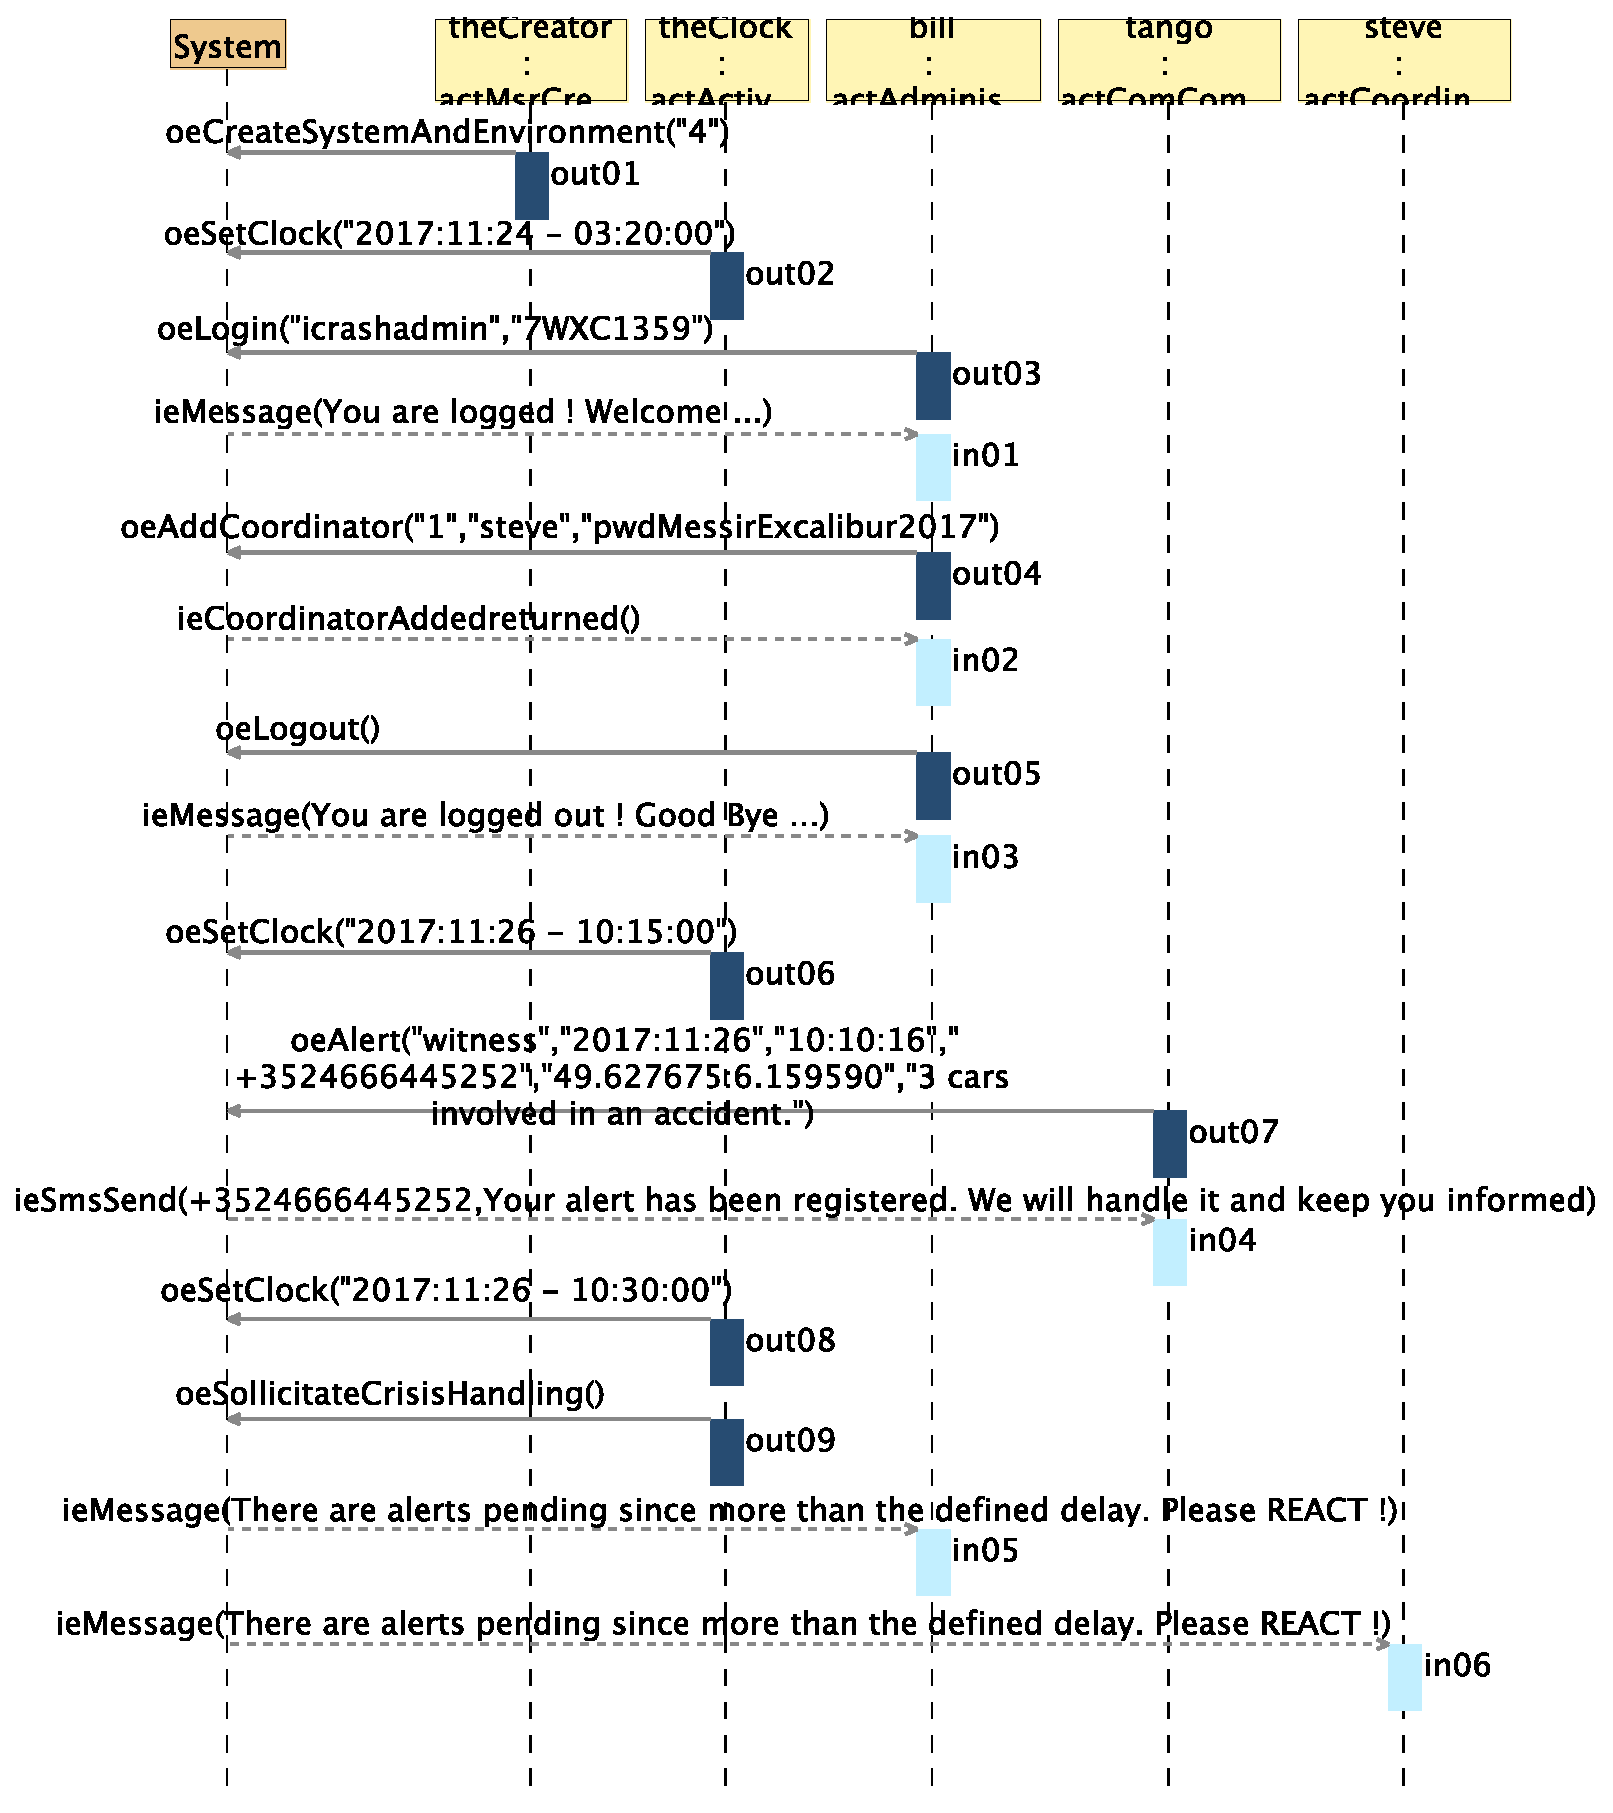
\includegraphics[
	angle=0
	,height=1.0\textheight
	]{./images-report-gen/usecase-model/summary/uci-suDeployAndRun-uciSimpleAndComplete-Part01.eps}
	\end{center}
	\caption[ru.iu.bachelor.sed.group01.icrash Sequence Diagram: uci-suDeployAndRun-uciSimpleAndComplete-Part01]{uci-suDeployAndRun-uciSimpleAndComplete-Part01
	}
	\label{fig:ru.iu.bachelor.sed.group01.icrash-RE-UC-uci-suDeployAndRun-uciSimpleAndComplete-Part01}
	\end{figure}
	\vspace{0.5cm}
